\section{Einleitung}
Diese Arbeit beschäftigt sich mit der automatischen Trennung von Schüttgutpartikel. Der Begriff Schüttgut bezeichnet hierbei ein körniges oder auch stückiges Gemenge, dass in einer schüttfähigen Form vorliegt (Wiki). Die Abbildung \ref{fig:Schuettgut} zeigt Schüttgut in unterschiedlicher Größe. In der Industrie werden heutzutage Schüttgüter maschinell auf Mängel geprüft und auch Schüttgüter mit unterschiedlichen Güteklassen maschinell getrennt. Anwendungsgebiete sind vor allem in der Essensindustrie, beim Recycling, dem Bergbau usw.. Im Vergleich zur Sortierung per Hand, welche subjektiv und unbeständig ist, hilft die maschinelle Sortierung die Produktqualität und den Durchsatz zu erhöhen, während Kosten reduziert werden \cite{FoodQuality}. 

\begin{figure}[!h]
    \centering
    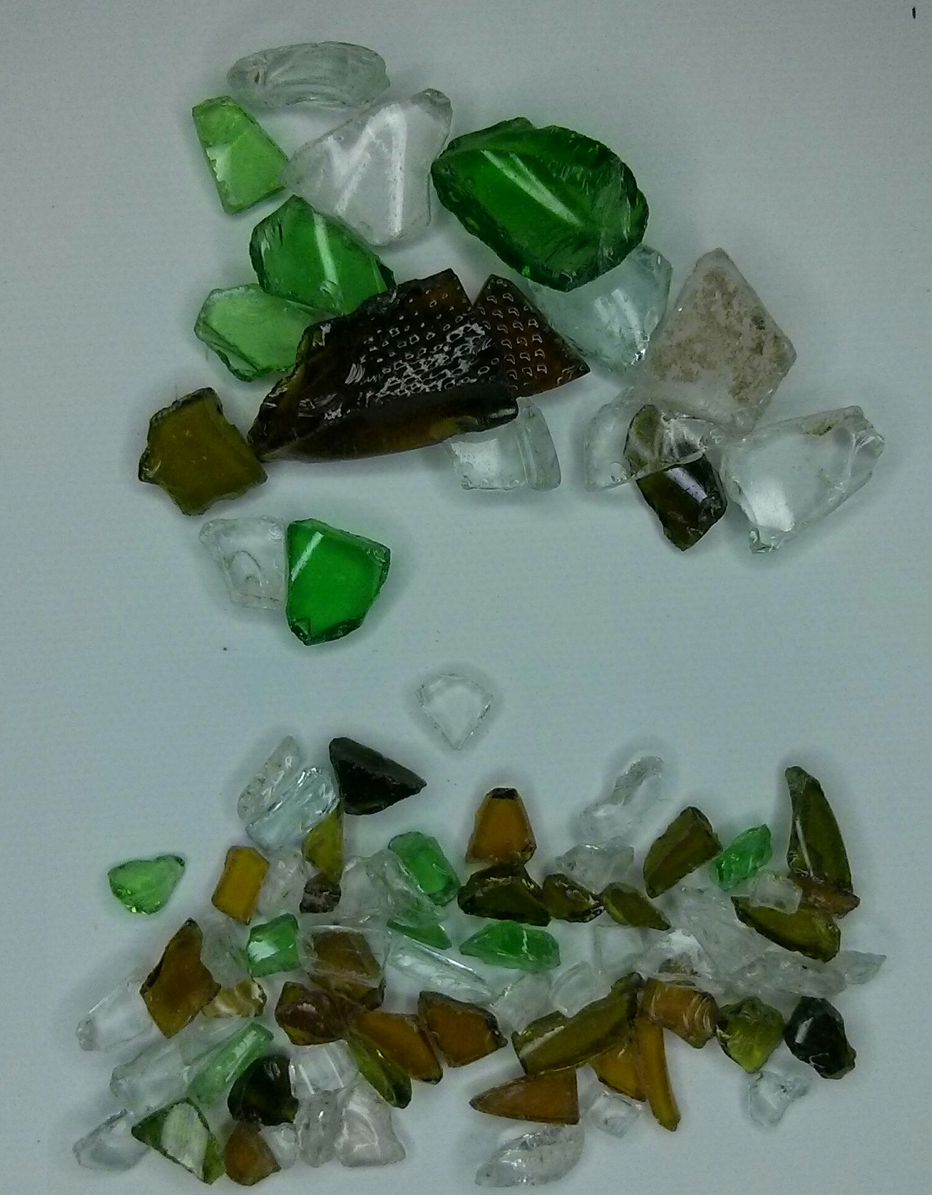
\includegraphics[width=0.3\textwidth]{pics/Schuettgut.png}
    \caption{Schüttgut}
    \label{fig:Schuettgut}
\end{figure}

\subsection{Der sensorbasierte Sortierprozess}
Der sensorbasierte Sortierprozess läuft im Allgemeinen wie in Abbildung \ref{fig:Aufbau} ab. Es wird Schüttgut portionsweise an den Anfang eines Fließbandes gestreut. Das Fließband mit beliebiger Länge beschleunigt die Partikel. Ein Sensor misst die Schüttgutpartikel auf dem Fließband. Aufgrund dieser Messung werden die Partikel am Ende des Fließbandes in bestimmte Behälter geleitet und so voneinander getrennt. 

Ein solcher Sensor kann beispielsweise eine Zeilenkamera oder eine Flächenkamera sein. Die Analyse jedes Partikels durch eine Zeilenkamera beschränkt sich dabei nur auf wenige Bildern. Dadurch ist eine Bewegungsanalyse nicht möglich. Durch geschickte Beleuchtung kann jedoch anhand von optischen Merkmalen eine Klassifikation ermöglicht werden. Mithilfe einer Flächenkamera kann hingegen ein Bewegungsverlauf aufgezeichnet und analysiert werden. Partikel unterscheiden sich hierbei nicht nur durch ihren auf dem Band zurückgelegten Pfad, sondern auch hinsichtlich der Geschwindigkeit in Bandrichtung und orthogonal zur Bandrichtung.

\begin{figure}[!h]
    \centering
    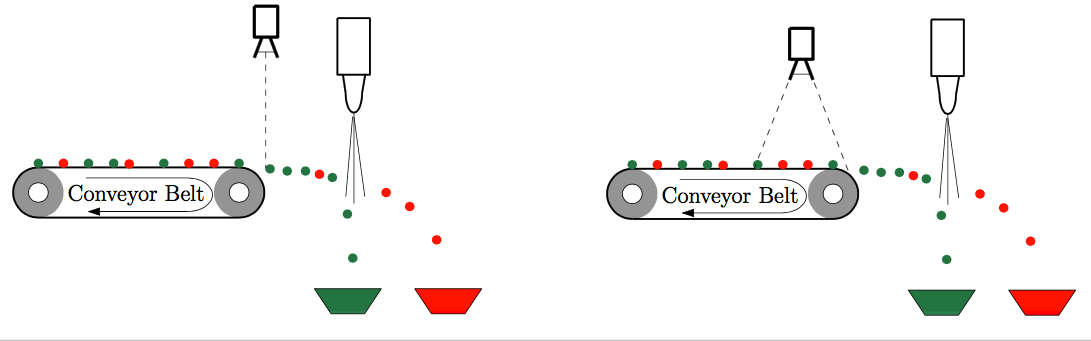
\includegraphics[width=0.7\textwidth]{pics/aufbau.png}
    \caption{Aufbau aus der MA}
    \label{fig:Aufbau}
\end{figure}

\subsection{Motivation}
Das Ziel dieser Arbeit ist es mithilfe einer Flächenkamera automatisch ein Schüttgut-Partikel abhängig von seinem Bewegungsverlauf zu klassifizieren. Das Erlernen einer akkuraten Klassifikation eines neuen bzw. unbekannten Schüttguts soll dabei schnell und einfach möglich sein. 

\subsection{Bisherige Arbeiten}
In der Arbeit (MA-Thesis) wurde gezeigt, dass auf Basis von Bewegungsmustern eine einfache Klassifikation von Objekten durchgeführt werden kann. Als Testdaten wurden dazu mehrere Objektarten verwendet, die drei Oberklassen zugeordnet werden können. Mithilfe eines naiven Bayes Klassifikator sollten die verschiedenen Objektarten einer der drei Oberklassen zugeordnet werden.

Da die Testdaten pro Objektart aber nur aus 52 Objekten bestanden, konnte kein repräsentative Likelihood Funktion umgesetzt werden (MA S.24). Außerdem wurde festgestellt, dass manche Objektarten sich sehr ähnlich verhalten. Unter der Berücksichtigung der genannten Einschränkungen konnten im Durchschnitt in 90\% der Fälle die Objekte der richtigen Oberklasse zugeordnet werden (MA S.24). Die Arbeit kommt zum Schluss, dass durch mehr Testdaten und Features ein besseres Klssifikationsergebnis erreicht werden kann.

\subsection{Zielsetzungen}
Es soll eine akkurate Klassifikation von mehr als 90\% bei allen Schüttgutarten gewährleistet sein. Dabei soll der Klassifikator nicht nur zwischen Oberklassen, sondern zwischen Basisklassen unterscheiden und wird damit weit über die Ergebnisse des MA-Thesis hinaus gehen. Der Klassifikator soll dazu möglichst wenige Realdaten benötigen und keine optischen Merkmalen, sondern ausschließlich Daten aus dem Bewegungsverlaufs verwenden. Die spätere Umsetzung des Klassifkators soll durch Optimierung der Anlagenparameter 
außerdem in Echtzeit möglich sein. 




